% This work is licensed under the Creative Commons Attribution-NonCommercial 4.0 International License.
% To view a copy of this license, visit http://creativecommons.org/licenses/by-nc/4.0/
% or send a letter to Creative Commons, PO Box 1866, Mountain View, CA 94042, USA.

% !TEX TS-program = xelatex

\documentclass[../Main/chem371-notes.tex]{subfiles}

\setcounter{chapter}{3}
\begin{document}

\chapter{Basis Sets}

In the previous chapter we introduced the Hartree--Fock method. 
The goal of this chapter is to discuss some practical aspects of how Hartree--Fock computations actually run on a computer and the way the are approximated.
We will encounter the idea of using a basis of functions (basis set) to find approximate solutions that can be systematically improved.
Lastly, we will look at some applications of these ideas.

\section{Exact solutions to the Schr\"{o}dinger equation}
As it was mentioned earlier, we know exact solutions of the Schr\"{o}dinger only for a handful of models.
An example that should be familiar to you is the hydrogen atom.
For this system, the solutions are known to depend on three quantum numbers $n$, $l$, and $m_l$, and that the energy levels (eigenvalues) are given by (in atomic units)
\begin{iequation}
E_n = - \frac{1}{2 n^2}  \, E_\mathrm{h}, \quad n = 1, 2, \ldots
\end{iequation}
The wave function $\psi_{nlm_l}$ is usually expressed in \emph{spherical coordinates} ($r, \theta, \phi$)\mnote{
If you are curious, spherical coordinates are connected to Cartesian coordinates via the following equations
\begin{align*}
x & =  r \sin \theta \cos \phi, \\
y & =  r \sin \theta \sin \phi, \\
z & =  r \cos \theta
\end{align*}
\centering{
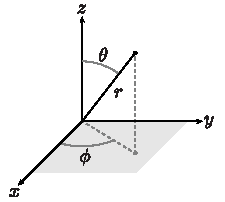
\includegraphics[width=2.0in]{img/spherical_coordinates.pdf}}
\captionof{figure}{Definition of the spherical coordinates $r$, $\theta$, and $\phi$.}
\label{fig:rigidrotor:spherical}
}
 as a product of a function that depends on the electron distance $R_{nl}(r)$ and a term that depends on the angles $\theta$ and $\phi$, which we write as $Y_l^{m_l}(\theta,\phi)$
\begin{equation}
\psi_{nlm_l}(r,\theta,\phi) = R_{nl}(r) Y_l^{m_l}(\theta,\phi)
\end{equation}
For example, the wave function for the  ground state of hydrogen, the 1s orbital, is given by
\begin{equation}
\mathrm{1s} = \psi_{1,0,0}(r,\theta,\phi) = R_{1,0}(r) Y_0^0(\theta,\phi) = 2 e^{-r} \frac{1}{\sqrt{4\pi}} = \frac{1}{\sqrt{\pi}} e^{-r}
\end{equation}
while the 2p$_{z}$ orbital is given by
\begin{align}
\mathrm{2p}_{z} &= \psi_{2,1,0}(r,\theta,\phi) = R_{2,1}(r) Y_1^{0}(\theta,\phi) =
\frac{1}{4\sqrt{2 \pi}}   r e^{-r/2} \cos \theta.
\end{align}

When we turn to more complicated systems, like atoms with more than one electron and molecules, the Schr\"{o}dinger equation becomes intractable and we have to turn to approximate numerical methods to solve it (recall Dirac's quote on this point).
This is what we will look into in the next section.

\section{Basis}

\mfigure{
\centering{
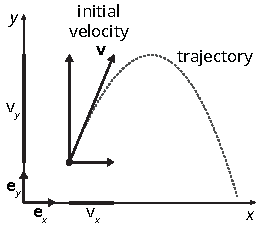
\includegraphics[width=1.75in]{img/trajectory.pdf}}
\captionof{figure}{The trajectory of a particle with initial velocity vector $\mathbf{v} = (v_x, v_y)$.
This vector may be decomposed in the basis of orthogonal unit vectors $\mathbf{e}_x$ and $\mathbf{e}_y$ as $\mathbf{v} = v_x \mathbf{e}_x + v_y \mathbf{e}_y$.}
\label{fig:2dtraj}
}

An important concept when constructing numerical approximations is that of a basis.
To build some intuition about the concept of a basis you can think back to your introductory physics courses and Newton's equations.
Consider the problem of describing the trajectory of a particle under the effect of gravity.
To solve this problem you need to specify the position and initial velocity of the particle.
The position can be specified by the $x$ and $y$ coordinates, and the initial velocity by the velocity in $x$ and $y$ directions ($v_x, v_y$).
These quantities are essentially vectors, which we indicate with the symbols $\mathbf{r} = (x,y)$ and $\mathbf{v} = (v_x,v_y)$. For example, the velocity vector $\mathbf{v}$ can be expressed as a sum of a component pointing in the $x$ direction ($\mathbf{e}_x$) and one pointing in the $y$ direction ($\mathbf{e}_y$)
\begin{equation}
\mathbf{v} = v_x \mathbf{e}_x + v_y \mathbf{e}_y
\end{equation}
The vectors $\mathbf{e}_x$ and $\mathbf{e}_y$ are called a \emph{basis}, because any vector in two dimensions $\mathbf{a}$ can be written as a sum of coefficients multiplied by the basis vectors
\begin{equation}
\mathbf{a} = a_x \mathbf{e}_x + a_y \mathbf{e}_y
\end{equation}
The vectors $\mathbf{e}_x$ and $\mathbf{e}_y$ have another special property: they are orthogonal, which means that their dot product is zero
\begin{equation}
 \mathbf{e}_x \cdot \mathbf{e}_y = 0.
\end{equation}

In the more general case, the velocity is a three dimensional vector, and must be described as a sum of three terms
\begin{equation}
\mathbf{v} = v_x \mathbf{e}_x + v_y \mathbf{e}_y + v_z \mathbf{e}_z
\end{equation}
Interestingly, this idea can also be extended to functions.
For example, suppose we want to approximate some function $g(x)$.
We could start from choosing two simple functions $f_1(x)$ and $f_2(x)$ and approximate $g(x)$ as
\begin{equation}
g(x) = c_1 f_1(x) + c_2 f_2(x)
\end{equation}



\section{Approximate solutions via expansion in a basis}
One way to find an approximate solution of the Schr\"{o}dinger equation is to express it as a \emph{linear combination of basis functions}.
This is a very common strategy for studying differential equations that are too difficult to solve in analytical form.
The basic idea is to approximate a function $g(x)$ as a sum of a finite number of fixed functions $f_i(x)$, called basis functions, multiplied by the coefficients $c_i$
\begin{equation}
g(x) \approx  c_1 f_1(x) +  c_2 f_2(x) + \cdots + c_K f_K(x) = \sum_{i=1}^{K} c_i f_i(x) 
\end{equation}
You can think of this approximation as fitting the function $g(x)$ with the basis functions, where the unknowns are the fitting coefficients $c_i$.
For example, we could choose the set of basis functions to be the polynomials of $x$ and stop at the polynomial of order $K$ (here we also include the constant term $x^0 = 1$)
\begin{equation}
g(x) \approx  c_0 +  c_1 x + \cdots + c_K x^{K} = \sum_{i=1}^{K} c_i x^{i-1}
\end{equation}

\mfigure{
\centering{
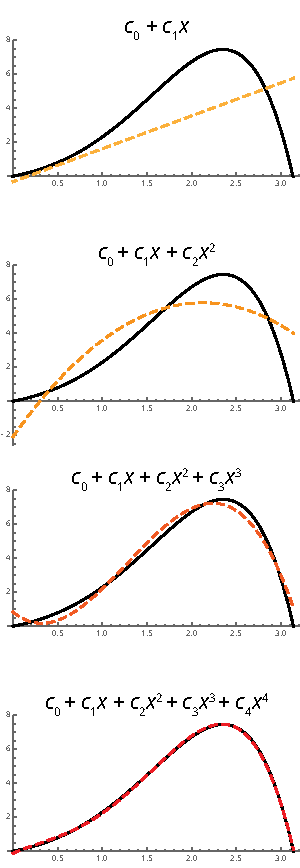
\includegraphics[width=1.75in]{img/basis_expansion.pdf}
}
\captionof{figure}{Example of expansion of the function $\exp(x) \sin(x)$ in a basis of polynomials $x^i$.
By the time we include fourth powers of $x$ this function is approximated well in the entire range $0 \leq x \leq \pi$.}
}

\section{Linear combination of atomic orbitals}

\centering{
\begin{tabular}{@{} cccc @{}} % Column formatting, @{} suppresses leading/trailing space
\toprule
Basis    & Basis Functions & Energy (\Eh) & Error (\Eh) \\
\midrule
cc-pVDZ &   5 & $-$0.499278403 & 0.000721597 \\ 
cc-pVTZ &  14 & $-$0.499809811 & 0.000190189 \\ 
cc-pVQZ &  30 & $-$0.499945569 & 0.000054431 \\ 
cc-pV5Z &  55 & $-$0.499994535 & 0.000005465 \\ 
cc-pV6Z &  91 & $-$0.499999245 & 0.000000755 \\ 
Exact &  $\infty$ & $-$0.500000000 & 0.000000000\\
\bottomrule
\end{tabular}
\captionof{table}{Convergence of the energy of the hydrogen atom as a function of the computational basis.
The exact solution corresponds to the analytic solution of the Schr\"{o}dinger equation.}
}

\centering{
\begin{tabular}{@{} ccc @{}} % Column formatting, @{} suppresses leading/trailing space
\toprule
Basis    & Basis Functions & Energy (\Eh) \\
\midrule
cc-pVDZ &  10 & $-$0.600264667 \\
cc-pVTZ &  28 & $-$0.602244426 \\
cc-pVQZ &  60 & $-$0.602520583 \\
cc-pV5Z & 110 & $-$0.602619758 \\
cc-pV6Z & 182 & $-$0.602632085 \\
\bottomrule
\end{tabular}
\captionof{table}{Convergence of the energy of the \ce{H2+} molecule at a bond distance $r_\mathrm{HH}$ = 2 bohr as a function of the computational basis.}
}


\end{document}